\documentclass[11pt,letterpaper]{article}
\usepackage{naaclhlt2015}
\usepackage{times}
\usepackage{latexsym}
\usepackage{url}
\usepackage[pdftex]{graphicx}
\usepackage{breqn}
\usepackage{multirow}
\setlength\titlebox{6.5cm}    % Expanding the titlebox

%%%%%%%%%%%%%%%%%%%%%%%%%%%%%%%%%%%%%%%%%%%%%%%%%%%%%%%%%%%%%%%%%%%%%%
% Code to use with NAACL/ACL style files to simulate natbib's 
% \citealt, which prints citations with no parentheses. This should
% work if pasted into the preamble. \cite, \newcite, and \shortcite
% should continue to work as before.

\makeatletter

\def\citealt{\def\citename##1{{\frenchspacing##1} }\@internalcitec}

\def\@citexc[#1]#2{\if@filesw\immediate\write\@auxout{\string\citation{#2}}\fi
  \def\@citea{}\@citealt{\@for\@citeb:=#2\do
    {\@citea\def\@citea{;\penalty\@m\ }\@ifundefined
       {b@\@citeb}{{\bf ?}\@warning
       {Citation `\@citeb' on page \thepage \space undefined}}%
{\csname b@\@citeb\endcsname}}}{#1}}

\def\@internalcitec{\@ifnextchar [{\@tempswatrue\@citexc}{\@tempswafalse\@citexc[]}}

\def\@citealt#1#2{{#1\if@tempswa, #2\fi}}

\makeatother
%%%%%%%%%%%%%%%%%%%%%%%%%%%%%%%%%%%%%%%%%%%%%%%%%%%%%%%%%%%%%%%%%%%%%%

% Effects of non-linguistic context
\title{Audience and discourse modulate information density on twitter 
% Information content changes with audience and conversation length in microblog texts
\Thanks{Thanks to...}}
% common ground decreases information

\author{Author 1\\
XYZ Company\\
111 Anywhere Street\\
Mytown, NY 10000, USA\\
{\tt author1@xyz.org}
	  \And
          Author 2\\
ABC University\\
900 Main Street\\
Ourcity, PQ, Canada A1A 1T2\\
{\tt author2@abc.ca}
}

\date{}


\begin{document}
\maketitle
\begin{abstract}
Optimal use of a noisy communication channel requires the uniform distribution of information across a message. The idea that language users might attempt to approximate this kind of optimal usage in their production is known as the ``uniform information density'' (UID) hypothesis. Previous work on UID has suggested that a signature of the hypothesis is an  increase in linguistic information across sentences in a text, presumably compensating for increasing shared context or common ground. We apply the UID hypothesis to data from a popular social media platform and find evidence for differences in information content across different audiences sizes for messages. In addition, we find an unpredicted effect: that information content decreases across small-audience conversations. We interpret these findings in terms of a noisy channel model in which smaller, more responsive audiences allow for message content to be distributed across multiple messages. 


\end{abstract}

\section{Introduction}

To make optimal use of a noisy communication channel, messages sent over the channel should have as close as possible to uniform information density (UID). If they do not, they either underutilize the channel or risk mistransmission \cite{levy2007}. Spoken and written language are clearly noisy channels for communication; do human language users use them optimally? The UID hypothesis is the conjecture that human language producers approximate uniformity in the information content of their messages. 
 
A growing body of work supports the UID hypothesis. There is clear evidence from phonology that speakers reduce more predictable sounds \cite{aylett2004,aylett2006,bell2003}, suggesting that they are giving more ``air time'' to less predictable material to equalize information density. And in syntax, speakers tend to drop optional materials (like the word ``that'' as a sentence-complementizer) in more predictable scenarios \cite{levy2007,frank2008,jaeger2010}, again implying a process of allocating communication time relative to predictability. Both of these sets of findings thus suggest at least some local sensitivity to message complexity.

Further evidence for the UID hypothesis comes from studies of the information content of linguistic materials across sequences of sentences. \citealt{genzel2002} showed that word-by-word complexity (measured by a standard n-gram language model) increases across sequences of sentences. They hypothesized that this increase was due to a corresponding increase in non-linguistic information that would make even more complex linguistic structures easier to predict. Follow-ups have shown that this same complexity increase effect is attested in different document types and across languages \cite{genzel2003,qian2012}. 

The presence and relative ubiquity of the complexity increase effect in written language allows it to be used as a tool to explore UID effects across domains. For example, recent work replicated this effect in the context of large-scale events (in this case, the World Series of Baseball) being discussed on the social media platform Twitter. That study found that that information density increased over the course of individual baseball games, suggesting that non-linguistic common ground drives differences in information density \cite{doyle2015}. Here we leverage this effect instead to explore differences in information density as a function of audience size---and related to this, overall channel capacity. 

Following \citealt{doyle2015}, we leverage Twitter to provide large amounts of text data relating to social interactions across many different scales. In particular, we take advantage of the fact that while messages on Twitter are uniformly public, the defaults of the network imply audiences of vastly different size for different messages. In particular, we distinguish hashtagged messages, which are often intended to reach a wide audience; standard visible tweets, which are viewed by default by a user's followers; and responses, which are visible primarily to those users who are mentioned directly (see below for more details). 

These three ``modes'' provide three different channels that potentially have very different capacities. In a long chain of replies, there is a strong expectation that the intended audience will read a particular message. In contrast, in visible and hashtagged tweets, users typically only get a single message to express themselves---due to the volume of tweets in popular conversations there is no guarantee that any user will see and connect two different messages.  Thus, independent of the UID hypothesis, we should potentially observe different information densities across audiences, as users pack more information into individual public tweets but spread their content across longer chains of replies.

In addition, however, the presence of reply chains also allows us to investigate UID in dialogic contexts through the complexity increase effect \cite{genzel2002}. Previous work has been based on written texts (often news reports that follow a particular, relatively stereotyped format).  With the exception of one preliminary study that provided a partial replication of the original complexity increase effect using the Switchboard corpus \cite{vega2009}, to our knowledge no work has explored how the dynamics of conversation interact with UID. 





\section{Corpus}

Randomly sampling conversations on a medium like Twitter is a difficult problem. Twitter users routinely use the medium to converse in smaller groups via the \@ mention functionality (described in more detail below). Yet such conversations are not uniformly distributed: A random sample of tweets---perhaps chosen because they contain the word ``the'' or a similarly common token \cite{doyle2014}---does not yield any density of dialogues. Dialogues tend to occur because a user with a sufficient community of followers posts a tweet that causes followers to engage and then responds to at least some of the followers' reactions. 

\paragraph{Seed strategy}

To sample such interactions, we developed a ``seed'' strategy where we identified popular twitter accounts and then downloaded a large sample of their tweets, then downloaded a sample of the tweets of all the users they mentioned. This strategy allowed us to reconstruct a relatively dense sample of dialogues (reply chains).

\begin{table}
\begin{center}
\begin{tabular}{|c|c|}
\hline
{\tt @camerondallas} & \multirow{2}{*}{Youtube celebrities} \\
{\tt @rickypdillon} & \\
\hline
{\tt @edsheeran} & \multirow{2}{*}{Musicians} \\
{\tt @yelyahwilliams} & \\
\hline
{\tt @felixsalmon} & \multirow{2}{*}{Journalists} \\
{\tt @tanehisicoates} & \\
\hline
{\tt @jahimes} & \multirow{3}{*}{Politicians} \\
{\tt @jaredpolis} & \\
{\tt @leezeldin} & \\
\hline
{\tt @larrymishel} & \multirow{2}{*}{Economists} \\
{\tt @paulnvandewater} & \\
\hline
{\tt @neiltyson} & \multirow{3}{*}{Pop. Scientists} \\
{\tt @profbriancox} & \\
{\tt @richardwiseman} & \\
\hline
\end{tabular}
\end{center}
\caption{\label{tab:seed-users} Seed users for our dataset.}
\end{table}

We began by choosing a set of 14 seed Twitter accounts that spanned a variety of genres, were popular enough to elicit replies, and interacted with other users often enough to build up a community.  The seed users are listed in Table \ref{tab:seed-users}.  

To build conversations, we needed to obtain tweets directed to and from these seed users. For each seed user, we downloaded their last 1500 tweets, extracted all users mentioned within those tweets, and downloaded each of their last 1500 tweets.  To capture tweets that failed to start conversations with the seed users, we also added the last 1000 tweets mentioning each seed user's handle.  Tweets that appeared in multiple communities were removed.  Each reply contains the ID of the tweet it replies to, so we could rebuild conversation trees back to their roots, so long as all of the preceding tweets were made by users in our communities.

\paragraph{Conversation structure and visibility}

Twitter conversations follow a basic tree structure with a unique root node. Each tweet is marked as a reply or not; for replies, the user and tweet IDs of the tweet it replies to is stored. Each tweet can be a reply to at most one other tweet, so a long conversation resembles a linked list with a unique root node. ``Mentions,'' the inclusion of a username in a tweet, are included in tweets by default throughout a conversation unless a tweeter chooses to remove some of them, so tweets deep in a conversation may be primarily composed of mentions rather than new information.

Mentions also affect tweet visibility.  Tweets whose first character is a mention (whether or not it is a reply) do not show up by default when browsing a user's tweets, unless the browser follows both the tweeter and first-mentioned user.\footnote{This behavior varies slightly depending on what application is used to view Twitter.  On the website, mention-first tweets do not appear in lists and only appear after clicking the 'tweets \& replies' option on a timeline. On the Twitter mobile app, mention-first tweets appear by default on a timeline but still not in lists.}

After some processing described below, this process resulted in 5.5 million tweets, of which 230,023 were part of rooted conversations with at least one reply in our dataset. An additional 3.3 million tweets were not part of a conversation (not a reply, and received no replies).  Unfortunately, Twitter only tracks replies up a tree, so while we know with certainty whether a tweet is a reply (even if it is to a user outside our communities), we do not know with certainty that a tweet has recieved no replies, especially from users outside our communities.  The remaining 2 million tweets were replies whose conversations could not be traced back to the root.


\paragraph{Information content estimation}

To estimate the information content of a tweet, we first tokenized the tweets using Twokenizer \cite{owoputi2013}. We then removed any number of mentions at the beginning or end of a tweet, as these are usually markers of conversation structure rather than conveying information themselves.  Tweet-medial mentions were retained but masked with the single type {\it [MENTION]}. Links were similarly masked as {\it [URL]}. Punctuation and emoji were retained.

We then built trigram langauge models using SRILM with default settings and Kneser-Ney discounting.  Types with fewer than 5 tokens were treated as out-of-vocabulary items. For each seed user, the training set was the set of all tweets from all other seed users.  

\section{Analyses}

We describe the results of three sets of analyses looking at the influence of audience size and available context on apparent informativity. The first examines the effect of expected audience size at a coarse level, comparing tweets directed at a small subset of users, all one's followers, or the wider realm of a hashtag.   The second examines the effect of finer differences in known audience size on apparent informativity.  The third moves into conversations and tracks how conversational context and length affect informativity.

[What's the right thing to call the perplexity? Apparent/out-of-context informativity? Predictability?]

\subsection{Expected audience size}
First, we consider three different types of tweets and their expected audience size.  A tweet whose first word is a mention will not appear in most Twitter visualizations unless the reader follows both the tweeter and the first-mentioned user, or is mentioned somewhere in the tweet. (We will refer to these as ``invisible'' tweets as they are invisible to followers by default.)  A tweeter making an initial-mention tweet thus should expect such a tweet to have a relatively limited audience, with a focus on the mentioned users.\footnote{As evidence for conscious manipulation of the audience size, many tweets have an initial period or other punctuation mark to prevent this hiding of a tweet, and some users will switch between initial-mention replies and ``dot''-replies in the course of a conversation to change the audience.}

On the other side, a hashtag serves as an ad hoc categorization mechanism, and often is used to expand the potential audience for a tweet by including in the feeds of users tracking that hashtag, regardless of whether they follow the tweeter.  Thus, a tweeter using a hashtag should expect a larger audience than normal.  Finally, we have baseline tweets which contain neither mentions nor hashtags and whose expected audience size is approximately one's followers.

Intuitively, context is higher for smaller audiences. Context should be highest for the invisible tweets, where the audience is limited and has seen or can access the previous tweets in the conversation.  Context should be lowest for the hashtagged tweets, where the audience is the largest and will likely contain many users who are completely unfamilair with the tweeter.  If contextualized UID is the driving force affecting information content, then the invisible tweets should have the highest entropy and hashtagged tweets should have the lowest.

Figure \ref{fig:audience-coarse} plots the entropy of tweets for these three audience sizes, and shows the opposite effect.  Per-word and per-tweet entropy both significantly {\it increase} with expected audience size ($p < .001$).

\subsection{Known audience size}
The results from expected audience size have a potential confound in that the way these different tweet types are accessed are sbstantially different, and may encourage different decision-theoretic choices in tweet behavior.  TWeets with mentions are highly likely to be seen by the mentioned user (unless the mentioned user is very commonly mentioned), whereas the likleihood of a given hashtagged tweet being seen through the hashtag-searching mechanism is very low.  This may lead a rational tweeter to package information into tweets differently, such as including more redundant information across tweets when the likleihood of any given tweet being read is low.

To assess audience size effects in a more controlled setting, we look at tweets with varying numbers of mentions.  Invisible tweets with few mentions have a smaller audience than invisible tweets with more mentions.  Visible tweets, on the other hand, have approximately the same audience size regardless of the number of mentions.  Therefore, we examine the effect of number of mentions in invisible tweets on entropy both in isolation and in comparison to the effect of the number of mentions in visible tweets.


\subsection{Reply depth and conversation length}
[Blah blah on why interesting.]

\begin{figure}
 \centering
  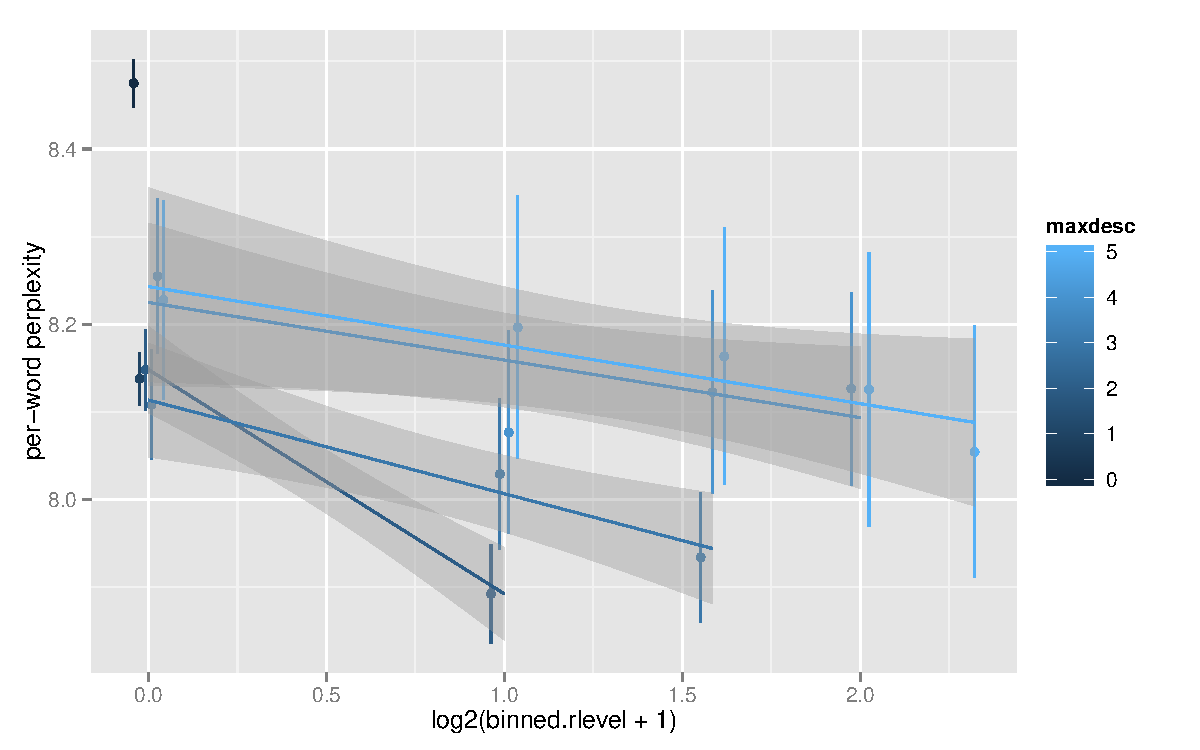
\includegraphics[width=3.25in]{figures/rlevel-and-maxdesc.pdf}
 \caption{Per-word entropy decreases with reply level and increases with maximum conversation depth. Linear fits with 95\% confidence intervals.}\label{fig:rlevel-maxdesc}\vspace*{-.5em}
\end{figure}


Figure \ref{fig:rlevel-maxdesc} plots mean perplexities for different reply levels and maximum conversation depths. Increasing the reply level decreases the information content of the tweet, while increasing the conversation depth increases the information content.

We fit a linear mixed-effects regression model to per-word and per-tweet perplexity.  Control factors were the logarithm of the tweet reply level and the logarithm of the maximum descendant level, along with a separate binary variable for whether the tweet was part of a conversation at all. A random by-user intercept was also included.  Both log reply level and log descendant level had significant effects by likelihood-ratio tests.

Reply level had negative effects on per-word and per-tweet perplexity (per-word: $-.341 \pm .009$; $p < .001, \chi^2(1) = 1466$, per-tweet: $-39.6 \pm .3$; $p < .001, \chi^2(1) =  16777$).

Maximum descendant level had positive effects on per-word and per-tweet perplexity (per-word: $.285 \pm .010$; $p < .001, \chi^2(1) = 817$, per-tweet: $35.1 \pm .3$; $p < .001, \chi^2(1) = 10520$).

Tweets that were not part of a conversation (non-reply tweets that generated no replies) had significantly higher perplexities than non-reply tweets that did generate at least one reply (per-word: $.379 \pm .008$; $p < .001, \chi^2(1) = 2035$, per-tweet: $29.4 \pm .3$; $p < .001, \chi^2(1) = 10372$).  

To summarize these effects, all conversations become more predictable as they go along. The longer the conversation goes, the less predictable it was to begin with, but the most unpredictable tweets fail to start a conversation at all.

\section{Discussion}

\subsection{Information decrease}
Why do Twitter conversations look different from the increasingly-informative texts studied in previous work? For one, these are true dialogues, whereas almost all of the sentence-level context informativity results were based on single-author texts.  Dialogues are often reactive; for instance, a reply may be a clarification question, which is likely to be shorter and more preictable than the original statement. Aside from rhetorical questions, single-author texts are unlikely to include such predictable reactions.

Furthermore, in most of the previously-studied genres, the authors of the texts could reasonably expect their readers to be both focused and unlikely to disengage from reading. Tweets, however, are often read and responded to while doing other tasks, reducing focus and increasing disengagement rates.  Interestingly, the one genre where \newcite{genzel2003} found a negative effect of sentence number on informativity was tabloid newspapers, whose authors can assume that their readers are likely to be distracted and to disengage prematurely.

This leads to a second question: does this contradict the core UID claim?  Common ground should rarely decrease over the course of a conversation, even in social media, and the ability to look back at previous statements within a written conversation should make common ground more stable as well.  The UID claim is based on a noisy-channel conception of communication, with humans attempting to operate near the channel capacity to maximize communication efficiency, and as shown by \newcite{genzel2002}, this implies that deconextualized estimates of entropy must go up as context increases.

One possibility is that conversational efficiency is not measured in linguistic information alone, and the UID hypothesis is not valid when linguistic information rate optimization is not the primary goal.  The last tweet in a Twitter conversation, for instance, often looks distinct from the previous tweets; often it is just a single word (e.g., {\it haha}) or an emoji/emoticon.  These are highly predictable, and have low information content whether estimated in or out-of-context.  However, they convey important meta-linguistic information (e.g., acknowledgment, approval), and simply omitting this or replacing it with a response that looks more like its predecessors is clearly sub-optimal behavior for a normal conversationalist.  [Show/mention result on rate of no-linguistic-info tweets by reply level?]

Another possibility is that the noisy-channel model should be tweaked for settings such as Twitter.  The locus of the noise in tweets centers on whether a reader gets the tweet and context at all.  Many Twitter users follow an enormous number of users, so outside of directed mentions and replies, there is a substantial chance that any given tweet will go unread by part of its intended audience. As a result, tweets may contain their own context; for instance, a user may talk about a recent event and include a link to an article about it.  

%\section*{Acknowledgments}
%
%We gratefully acknowledge the support of ONR Grant N00014-13-1-0287.

\newpage

\bibliographystyle{naaclhlt2015}
\bibliography{tweetdiscourse}

\end{document}